30. Марина ходит в спортзал один раз в 6 дней, Маша --- один раз в 3 дня, а Катя --- один раз в 4 дня. Они встретились в спортзале в субботу. В какой день недели они встретятся вновь?
\newpage
\noindent31. Расставьте в клетках данной таблицы числа 4, 5, 6, 7, 8, 9, 10, 11, 12 (по одному каждое) так, чтобы сумма чисел в каждой строке, каждом столбце и на двух главных диагоналях была равна 24.
\begin{center}
\begin{figure}[ht!]
\center{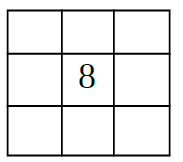
\includegraphics[scale=0.35]{5.png}}
\end{figure}
\end{center}
